\section{Robust Regression}

\subsection{Recommended References}
\begin{frame}{Recommended References}
	\begin{vfilleditems}
		\item \textcite{gelman2013bayesian} - Chapter 17: Models for robust inference
		\item \textcite{mcelreath2020statistical} - Chapter 12: Monsters and Mixtures
		\item \textcite{gelman2020regression}:
		\begin{vfilleditems}
			\item Chapter 15, Section 15.6: Robust regression using the t model
			\item Chapter 15, Section 15.8: Going beyond generalized linear models
		\end{vfilleditems}
	\end{vfilleditems}
\end{frame}

\begin{frame}{Robust Models\footnote{\href{https://github.com/allisonhorst/stats-illustrations}{figure from Allison Horst (CC-BY-4.0)}.}}
	\begin{columns}
		\begin{column}{0.6\textwidth}
			Almost always data from real world are really strange.
			\vfill
			For the sake of convenience, we use simple models.
			But always ask yourself.
			How many ways might the posterior inference depends on the following:
			\vfill
			\begin{vfilleditems}
				\item extreme observations (outliers)?
				\item unrealistic model assumptions?
			\end{vfilleditems}
		\end{column}
		\begin{column}{0.4\textwidth}
			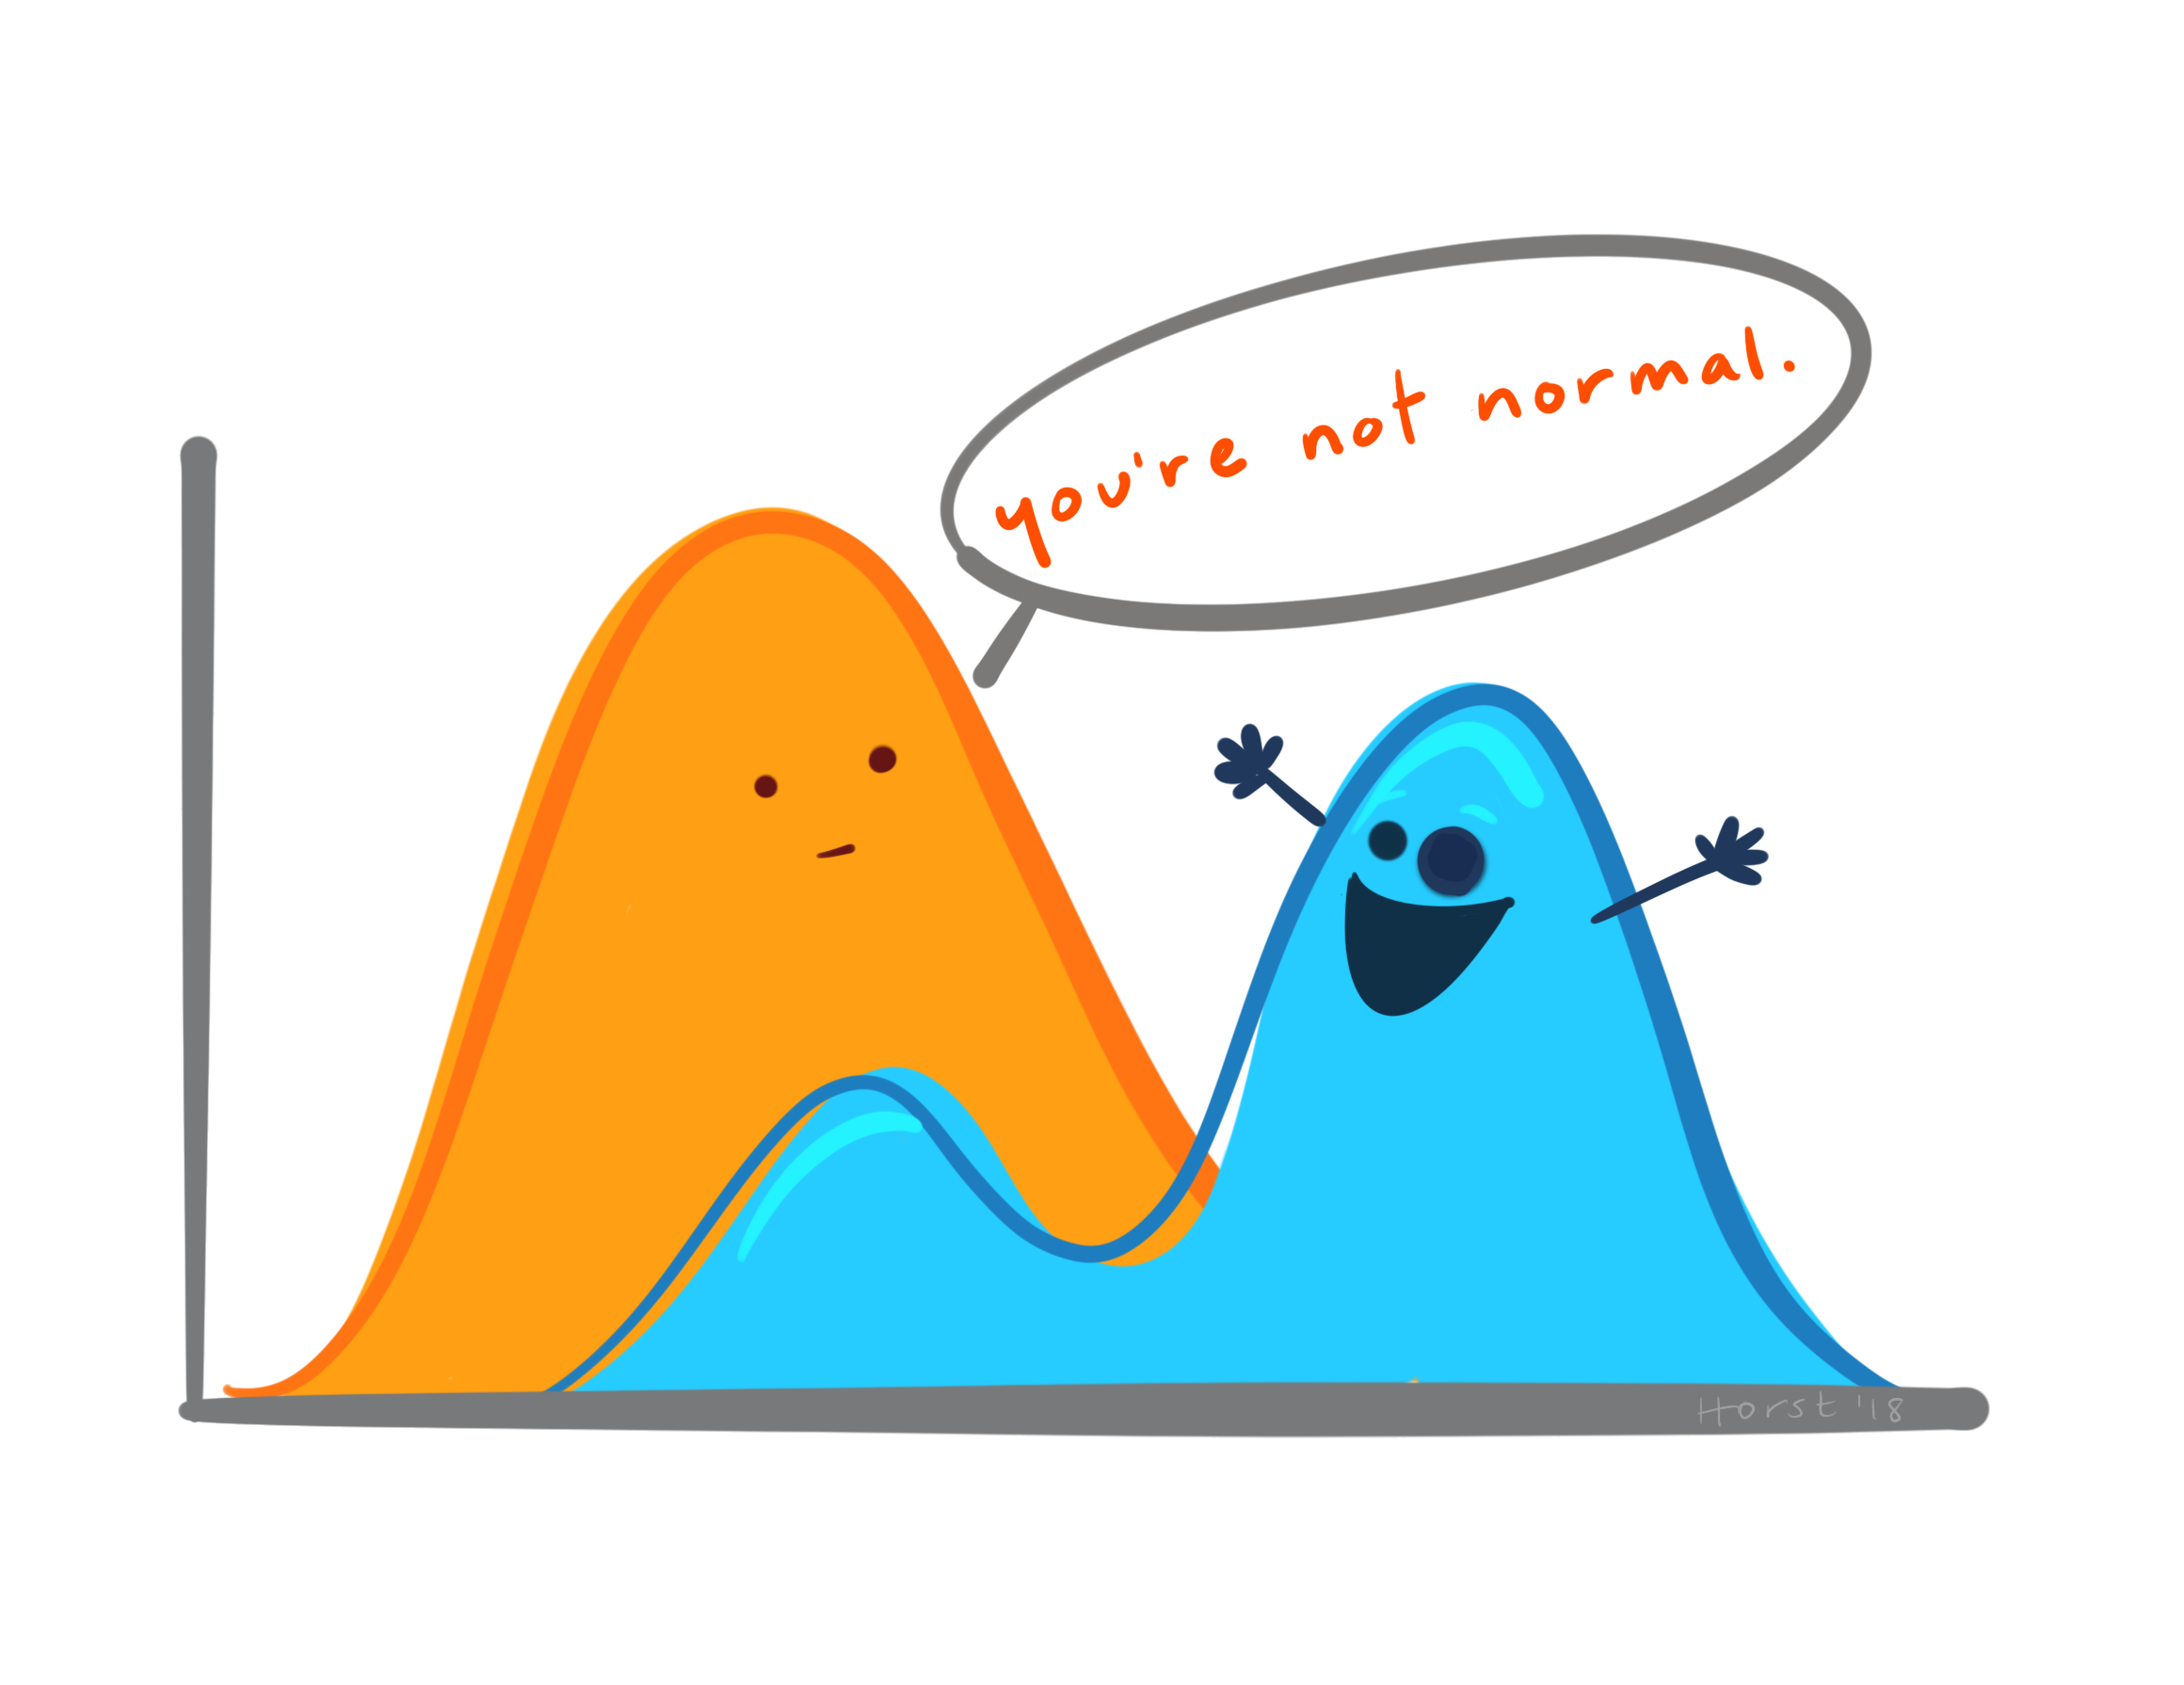
\includegraphics[width=0.9\columnwidth]{not_normal_transparent.png}
		\end{column}
	\end{columns}
\end{frame}

\subsection{Outliers}
\begin{frame}{Outliers}
	Models based on the \textbf{normal distribution are notoriously ``non-robust''
		against outliers},
	in the sense that a \textbf{single observation can greatly affect the
		inference of all model's parameters},
	even those that has a shallow relationship with it.
\end{frame}

\subsection{Overdispersion}
\begin{frame}{Overdispersion}
	\begin{defn}[Overdispersion and underdispersion]
		Superdispersion and underdispersion\footnote{
			rarer to find in the real world.}
		refer to data that have more or fewer variation than expected
		under a probability model.
		\parencite{gelman2020regression}
	\end{defn}
	\vfill
	For each one of the models we covered, there is a \textbf{natural extension}
	in which \textbf{a single parameter} is added to allow for overdispersion.
	\parencite{gelman2013bayesian}.
\end{frame}

\begin{frame}{Overdispersion Example}
	\begin{example}[Car accidents]
		Suppose you are analyzing data from car accidents.
		The model we generally use in this type of phenomena is
		\textbf{Poisson regression}.
		\vfill
		Poisson distribution has the same parameter for both the mean and variance:
		the rate parameter $\lambda$.
		\vfill
		Hence, if you find a higher variability than expected under the
		Poisson likelihood function allows,
		then probably you won't be able to model properly the desired phenomena.
	\end{example}
\end{frame}

\subsection{Overdispersion Versions of Probabilistic Models}
\subsubsection{Student's $t$ instead of the Normal}
\begin{frame}{Student's $t$ instead of the Normal}
	Student's $t$ distribution has \textbf{wider\footnote{or ``fatter''.} tails}
	than the Normal distribution.
	\vfill
	This makes it a good candidate to \textbf{fit outliers without
		instabilities in the parameters' inference}.
	\vfill
	From the Bayesian viewpoint, there is nothing special or magical in the
	Gaussian/Normal likelihood.
	It is just another distribution specified in a statistical model.
	We can make our model robust by using the Student's $t$ distribution
	as a likelihood function.
\end{frame}

\begin{frame}{Student's $t$ instead of the Normal}
	\centering
	\begin{tikzpicture}
		\begin{axis}[every axis plot, line width=2pt,
				ylabel=PDF,
				domain=-4:4,samples=200,
				axis x line*=bottom, % no box around the plot, only x and y axis
				axis y line*=left % the * suppresses the arrow tips
			]

			\addplot [blue] {gaussian(0, 1)};
			\addlegendentry{Normal}
			\addplot [red] {student(3)};
			\addlegendentry{Student's $t$ with $\nu=3$}
		\end{axis}
	\end{tikzpicture}
\end{frame}

\begin{frame}{Student's $t$ instead of the Normal}
	By using a Student's $t$ distribution instead of the Normal distribution
	as likelihood functions,
	the model's error $\sigma$ does \textit{not} follow a Normal distribution,
	but a Student's $t$ distribution:
	$$
		\begin{aligned}
			\boldsymbol{y}     & \sim \text{Student}\left( \nu, \alpha + \mathbf{X} \boldsymbol{\beta}, \sigma \right) \\
			\alpha             & \sim \text{Normal}(\mu_\alpha, \sigma_\alpha)                                         \\
			\boldsymbol{\beta} & \sim \text{Normal}(\mu_{\boldsymbol{\beta}}, \sigma_{\boldsymbol{\beta}})             \\
			\nu                & \sim \text{Log-Normal}(2, 1)                                                          \\
			\sigma             & \sim \text{Exponential}(\lambda_\sigma)
		\end{aligned}
	$$
	\small
	Note that we are including an extra parameter $\nu$,
	which representes the Student's $t$ distribution degrees of freedom,
	to be estimated by the model \parencite{gelman2013bayesian}.
	This controls how wide or narrow the ``tails'' of the distribution will be.
	A heavy-tailed, positive-only prior is advised.
\end{frame}

\subsubsection{Beta-Binomial instead of the Binomial}
\begin{frame}{Beta-Binomial instead of the Binomial}
	The binomial distribution has a practical limitation that we only have
	one free parameter to estimate\footnote{since $n$ already comes from data.} ($p$).
	This implies in the \textbf{variance to determined by the mean}.
	Hence, the binomial distribution \textbf{cannot} tolerate overdispersion.
	\vfill
	A robust alternative is the \textbf{beta-binomial distribution}, which,
	as the name suggests, is a \textbf{beta mixture of binomials distributions}.
	Most important, it \textbf{allows that the variance to be independent of the mean},
	making it \textbf{robust against overdispersion}.
\end{frame}

\begin{frame}{Beta-Binomial instead of the Binomial}
	The \textbf{beta-binomial distribution} is a binomial distribution, where
	the probability of success $p$ is parameterized as a $\text{Beta}(\alpha, \beta)$.
	\vfill
	Generally, we use $\alpha$ as the binomial's probability of the success $p$,
	and $\beta$\footnote(sometimes specified as $\phi$) is the additional parameter
	to control and allow for overdispersion.
	\vfill
	Values of $\beta \geq 1$ make the beta-binomial behave the same as a binomial.
\end{frame}

\begin{frame}{Beta-Binomial instead of the Binomial}
	$$
		\begin{aligned}
			\boldsymbol{y}     & \sim \text{Beta-Binomial}(n, p, \phi)                                     \\
			p                  & \sim \text{Logística/Probit}(\alpha +  \mathbf{X} \boldsymbol{\beta})     \\
			\alpha             & \sim \text{Normal}(\mu_\alpha, \sigma_\alpha)                             \\
			\boldsymbol{\beta} & \sim \text{Normal}(\mu_{\boldsymbol{\beta}}, \sigma_{\boldsymbol{\beta}}) \\
			\phi               & \sim \text{Exponential}(1)
		\end{aligned}
	$$
	\vfill
	It is also proper to include the overdispersion $\beta$ parameter as an
	additional parameter to be estimated by the model
	\parencite{gelman2013bayesian,mcelreath2020statistical}.
	A heavy-tailed, positive-only prior is advised.
\end{frame}

\subsubsection{Student's $t$ instead of the Binomial}
\begin{frame}{Student's $t$ instead of the Binomial}
	\small
	Also known as Robit\footnote{there is a great discussion between
		Gelman, Vehtari and Kurz at
		\href{https://discourse.mc-stan.org/t/robit-regression-not-robust/21245/}{
			\texttt{Stan}'s Discourse}} \parencite{gelman2013bayesian, gelman2020regression}.
	The ideia is to make the logistic regression robust by using a
	\textbf{latent variable $z$} as the linear predictor.
	$z$'s errors, $\epsilon$, are distributed as a Student's $t$ distribution:
	A ideia é "robustizar"~ a regressão logística com uma formulação usando dados
	latentes $z$ e dar uma uma distribução $t$ de Student aos erros latentes $\epsilon$:
	$$
		\begin{aligned}
			y_i        & = \begin{cases} 0 & \text{se } z_i < 0 \\ 1 & \text{se }\ z_i > 0 \end{cases} \\
			z_i        & = X_i \boldsymbol{\beta} + \epsilon_i                                         \\
			\epsilon_i & \sim \text{Student} \left (\nu, 0, \sqrt{\frac{\nu - 2}{\nu}} \right)         \\
			\nu        & \sim \text{Gamma}(2, 0.1) \in \left[2, \infty \right)
		\end{aligned}
	$$
	\footnotesize
	O grande segredo aqui é usar uma distribuição Gamma como \textit{priori}
	dos graus de liberdade $\nu$ truncada para valor mínimo de $\nu = 2$. Outra opção
	é literalmente especificar $\nu=4$.
\end{frame}

% \begin{frame}[fragile]{\href{https://paul-buerkner.github.io/brms/}{\texttt{brms}} -- $t$ de Student ao invés da Binomial}
% 	\begin{lstlisting}[basicstyle=\footnotesize]
% stan_inv_robit <- "
% real inv_robit(real y, real nu) {
%     return(student_t_cdf(y, nu, 0, sqrt((nu - 2) / nu)));
%     }"
% stanvar_inv_robit <- stanvar(scode = stan_inv_robit, block = "functions")
% robit_formula <-
% bf(y_c | trials(1) ~ inv_robit(eta, nu),
%     nlf(eta ~ b0 + b1 * x),
%     b0 + b1 ~ 1,
%     nu ~ 1,
%     nl = TRUE)
% brm(formula = robit_formula,
%     family = @binomial("identity")@,
%     formula = robit_formula,
%     prior = c(prior(normal(0, 1), nlpar = b0),
%     prior(normal(0, 1), nlpar = b1),
%     prior(gamma(2, 0.1), nlpar = nu, @lb = 2@)),
%     stanvars = stanvar_inv_robit)
%     \end{lstlisting}
% \end{frame}

% \subsubsection{Binomial Negativa ao invés de Poisson}
% \begin{frame}{Binomial Negativa ao invés de Poisson}
% 	Esse é o exemplo que falamos sobre superdispersão.
% 	A distribuição de Poisson possui o mesmo valor como média e variância.
% 	\vfill
% 	Então, se você encontrar superdispersão, provavelmente precisará de uma alternativa
% 	robusta à Poisson. Aqui que entra a binomial negativa que "robustiza"~
% 	a Poisson com um parâmetro extra $\phi$.
% 	\vfill
% 	Esse parâmetro é a probabilidade de sucessos $p$ da distribuição binomial negativa
% 	e geralmente usamos uma distribuição gamma como \textit{priori} para que $\phi$
% 	cumpra a função de um parâmetro de~"dispersão recíproca".
% \end{frame}

% \begin{frame}{Binomial Negativa ao invés de Poisson}
% 	$$
% 		\begin{aligned}
% 			\boldsymbol{y}     & \sim \text{Binomial Negativa} \left( e^{(\alpha + \mathbf{X} \boldsymbol{\beta})}, \phi \right) \\
% 			\phi               & \sim \text{Gamma}(0.01, 0.01)                                                                   \\
% 			\alpha             & \sim \text{Normal}(\mu_\alpha, \sigma_\alpha)                                                   \\
% 			\boldsymbol{\beta} & \sim \text{Normal}(\mu_{\boldsymbol{\beta}}, \sigma_{\boldsymbol{\beta}})
% 		\end{aligned}
% 	$$
% 	A ideia é dar uma \textit{priori} cauda longa para $\phi$, algo como
% 	$\text{Gamma}(0.01, 0.01)$ funciona.
% \end{frame}

% \begin{frame}[fragile]{\href{https://paul-buerkner.github.io/brms/}{\texttt{brms}} -- Binomial Negativa ao invés de Poisson}
% 	\begin{lstlisting}
%     brm(...
%       family = @negbinomial(link = "log")@
%     )
%     \end{lstlisting}
% \end{frame}

% \subsubsection{Mistura de Binomial Negativa ao invés de Poisson}
% \begin{frame}{Mistura de Binomial Negativa ao invés de Poisson}
% 	\small
% 	Mesmo usando uma binomial negativa, caso a superdispersão seja muito acentuada,
% 	em especial quando temos muita \textbf{inflação de zeros} (\textit{zero-inflated}),
% 	o seu modelo ainda pode resultar em patologias.
% 	Uma outra sugestão é usar uma mistura de binomial negativa \parencite{mcelreath2020statistical}.
% 	Aqui, $S_i$ é uma variável binária (\textit{dummy})
% 	indicando se a observação $i$ tem valor diferente de zero ou não.
% 	$S_i$ pode ser modelado usando uma regressão logística:
% 	$$
% 		\begin{aligned}
% 			\boldsymbol{y}
% 			                    & \begin{cases}
% 				                      = 0,                                                                                             & \text{ se } S_i = 0 \\
% 				                      \sim \text{Binomial Negativa} \left( e^{(\alpha + \mathbf{X} \boldsymbol{\beta})}, \phi \right), & \text{ se } S_i = 1
% 			                      \end{cases} \\
% 			P(S_i = 1)          & = \text{Logística/Logit}(\mathbf{X} \boldsymbol{\gamma})                                                               \\
% 			\boldsymbol{\gamma} & \sim \text{Beta}(1, 1)
% 		\end{aligned}
% 	$$
% 	\small
% 	$\boldsymbol{\gamma}$ é um novo conjunto de coeficientes para essa parte do modelo com
% 	\textit{prioris} uniformes de $\text{Beta} (1, 1)$.
% \end{frame}

% \begin{frame}[fragile]{\href{https://paul-buerkner.github.io/brms/}{\texttt{brms}} -- Mistura de Binomial Negativa ao invés de Poisson}
% 	\begin{lstlisting}
%     brm(...
%       family = @zero_inflated_negbinomial(link = "log")@,
%       prior = c(
%           ...
%         @prior(gamma(0.01, 0.01), class = shape)@,
%         @prior(beta(1, 1), class = zi)@
%     ))
%     \end{lstlisting}
% \end{frame}

% \subsection{Por quê usar Modelos Não-Robustos?}
% \begin{frame}{Por quê usar Modelos Não-Robustos?}
% 	O \textbf{teorema do limite central} nos diz que a distribuição \textbf{normal}
% 	é uma modelo apropriado para dados que são formados como a \textbf{soma de um grande número
% 		de componentes independentes}.
% 	\vfill
% 	Mesmo quando não estão naturalmente implícitos na estrutura de um problema,
% 	os \textbf{modelos simples não-robustos são computacionalmente convenientes}.
% 	\vfill
% 	Claro o que deve sempre guiar a sua escolha de modelo, além da natureza específica
% 	do processo de geração de dados do fenômeno que você está estudando, é
% 	a \textbf{verificação preditiva da posterior}.
% \end{frame}
